\documentclass[../main.tex]{subfiles}
\begin{document}
\chapter{Stato dell'arte}

In questo capitolo verranno discussi i principali lavori che sono stati fatti durante l'ultimo decennio in letteratura. Si procede col fornire un'introduzione preliminare sui concetti che verranno utilizzati durante questa tesi.

\section{Malware}
Il termine malware è una combinazione delle parole \textit{malicious} e \textit{software}. Il malware rappresenta quei programmi software progettati per danneggiare o effettuare azioni indesiderate su un sistema informatico. \cite{MalwareDef}

Gli obiettivi che può avere un malware sono molteplici e sono in continua evoluzione. Il malware, a seconda dello scopo per cui è stato creato e alle sue caratteristiche, viene classificato nei seguenti modi:

\begin{verse}
				\textbf{Virus} Prendono il nome dai virus in campo biologico e si comportano in modo analogo, sono programmi che si replicano sul computer che hanno infettato e si predispongono ad infettare nuovi computer mediante mezzi di trasmissione quali email e chiavette USB. \cite{VirusDef}
\end{verse}

\begin{verse}
				\textbf{Spyware} Il termine Spyware è una combinazione delle parole \textit{Spy} e \textit{Software}. È un software che viene installato sul computer della vittima a sua insaputa e che raccoglie informazioni. 
				Uno spyware è oggetto di controversia perchè può essere utilizzato negli ambienti lavorativi per controllare le ricerche dei dipendenti o per controllare l'attività dei propri figli su internet. Anche se utilizzato per scopi più innocui può comunque violare la privacy dell'utente. \cite{Spyware2} \newline
				Usi più scorretti di programmi spyware prevedono di tracciare la cronologia internet di un utente per inviare pubblicità mirata, accedere alle password degli account in uso sul computer infetto e/o alle informazioni bancarie. Le informazioni raccolte attraverso l'uso di spyware possono essere utilizzate in vari modi, l'uso più frequente e più remunerativo ad oggi è quello di rivendere tali informazioni a dei terzi. \cite{Spyware1}
\end{verse}

\begin{verse}
				\textbf{Backdoor} Tradotto letteralmente come \textit{porta sul retro}, è un metodo utilizzato per avere un accesso privilegiato e spesso segreto che aggira il sistema di autenticazione previsto. Lo scopo di una backdoor è quello di permettere una connessione in remoto al computer vittima per prenderne il controllo.				
\end{verse}

\begin{verse}
				\textbf{Trojan} Il cavallo di Troia fu una macchina da guerra che, secondo la leggenda, fu usata dai greci per espugnare la citta di Troia. Questo termine è entrato nel linguaggio comune per indicare uno stratagemma con cui penetrare le difese. Nell'ambito dei malware il trojan è un software che si nasconde all'interno di un altro programma all'apparenza innocuo e che, se eseguito, esegue anche il codice del trojan \cite{TrojanDef}.
				Oggi col termine trojan ci si riferisce principalmente ai malware ad accesso remoto. Spesso vengono utilizzati per installare backdoor sui sistemi bersaglio. \cite{TrojanPurpose}
\end{verse}

I malware erano inizialmente usati per compiere azioni dolose sia da hacker malintenzionati che dai governi per sottrarre informazioni personali, inviare spam e commettere frodi. \cite{ScopoMalware} \cite{MalwareRevolution}

L'evoluzione e lo sviluppo di internet hanno portato ad un incremento degli utenti connessi sempre maggiore. Questa crescita di internet ha spostato l'obiettivo dei malware che vengono usati sempre di meno per compiere azioni dolose. Fin dal 2003 la maggior parte dei malware sono stati creati per prendere il controllo dei computer dell'utente vittima per scopi illeciti \cite{MalwareRevolution}. Vengono usati computer zombie per l'invio di email di spam o per effettuare attacchi distribuiti Denial of Service (DDoS).


\section{Botnet}
Nella sua forma più semplice una Botnet è un gruppo di computer che sono stati infettati da un malware che consente al suo controller, detto anche master, di avere il controllo sulle macchine infettate. Le Botnet sono usate dal master per compiere operazioni illecite ad insaputa della vittima. Una volta infetto, il computer della vittima prende il nome di zombie. \cite{Botnet} \newline
Per aggiungere un computer ad una botnet si infetta il computer vittima con un malware che installa una backdoor in grado di consentire al master di avere accesso remoto al computer infettato dal malware.
Il master ha così accesso ad un sistema gigantesco di computer zombie pronti ad essere attivati ed eseguire i suoi ordini. Le botnet rilevate e studiate nella storia dimostrano come questi sistemi possano arrivare a contenere anche milioni di computer infetti. \cite{Botnet}

I componenti di una botnet sono i seguenti:

\begin{verse}
				\textbf{Master} Il master è il computer che ha creato la botnet e che ne ha il controllo remoto. È detto C\&C (Command and Control) il programma che dà i comandi da eseguire tramite un canale nascosto sul computer della vittima.
\end{verse}

\begin{verse}
				\textbf{Control protocol} Il protocollo utilizzato dal master per comunicare con i computer zombie.
\end{verse}

\begin{verse}
				\textbf{Computer zombie} Computer connesso ad internet che è stato infettato attraverso dei virus o trojan e che può essere utilizzato in modo remoto. 
\end{verse}

Nella figura seguente viene rappresentato una possibile architettura di una botnet. Il master è il computer che controlla in modo remoto i computer zombie attraverso dei server C\&C.
\begin{figure}[H]
				\centering
				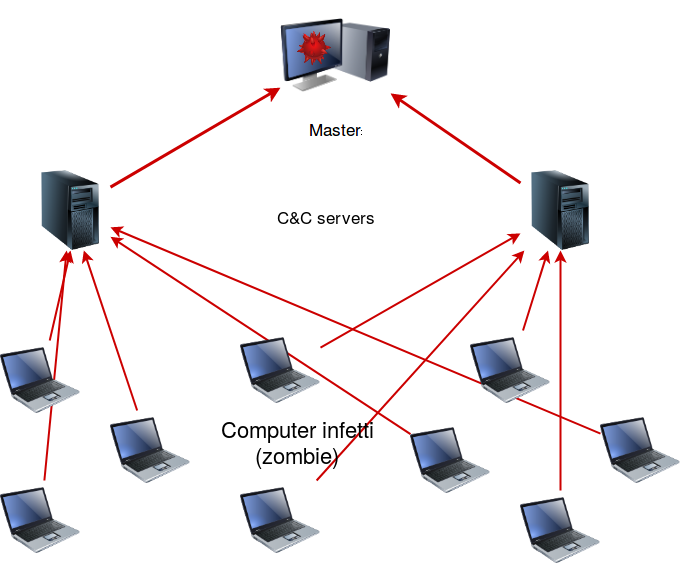
\includegraphics[scale=0.5]{botnet.png}
				\caption{Esempio architettura botnet}
\end{figure}

I principali attacchi informatici effettuati attraverso l'utilizzo delle botnet sono vari: possono essere spam, DDoS, click fraud, phishing e bitcoin mining per citarne alcuni. È quindi evidente come l'utilizzo delle botnet sia al fine di un guadagno economico.

\begin{verse}
				\textbf{Spam} È l'invio tramite posta elettronica di messaggi ad alta frequenza contenenti truffe o pubblicità.
\end{verse}

\begin{verse}
				\textbf{DDoS} Acronimo di Distributed Denial of Service, è un tipo di attacco in cui si mira a far esaurire le risorse di un sistema informatico affinchè non riesca più a fornire servizio. Per fare ciò si effettuano moltissime richieste al sistema per farlo rallentare o nei casi più estremi rendere inutilizzabile.
\end{verse}

\begin{verse}
				\textbf{Click fraud} Questo tipo di frode si verifica sulla pubblicità su internet di tipo pay per click. Questo tipo di pubblicità genera quantità di denaro in base al numero di click effettuati sull'annuncio pubblicitario. Le botnet sfruttano questo tipo di pubblicità utilizzando computer zombie per cliccare in massa gli annunci pubblicitari.
\end{verse}

\begin{verse}
				\textbf{Phishing} Con l'aumento di transazioni effettuate su internet il phishing è diventato sempre più comune \cite{phishing}. Il phishing è un tipo di truffa utilizzato per ottenere informazioni da utenti non esperti attraverso l'impesonazione di fonti attendibili \cite{phishingdef}.
\end{verse}

\begin{verse}
				\textbf{Bitcoin mining} I bitcoin sono una criptovaluta che a differenza dei soldi, che vengono stampati da un governo centrale, vengono creati risolvendo operazioni matematiche complesse. Una botnet utilizza i computer zombie come unità di calcolo a cui far eseguire queste operazioni complesse.
\end{verse}

\section{Botnet Detection}
Le botnet sono diventate il metodo preferito per lanciare attacchi su internet, sono una seria minaccia poichè possono inviare malware in modo coordinato e istantaneo da numerosi bot \cite{botnetdetection}.
Gli attacchi perpetrati dalle botnet si distinguono per il volume del traffico dati e per la velocità con cui sono commessi, questi attacchi riducono in modo significativo i tempi di risposta per difendersi.

È stimato che ci sono milioni di bot su internet ogni giorno, è quindi chiaro che le botnet sono diventate la minaccia più seria per la sicurezza su internet \cite{botnetdetection}.

Sono vari i metodi per cercare di individuare botnet su internet, quello che si è visto in questa tesi è basato sul modello comportamentale.
\begin{verse}
				\textbf{Botnet detection based on Network Behavior} Presenta un approccio per identificare le attività di C\&C delle botnet utilizzando le statistiche dei flow di rete come la larghezza di banda e la tempistica dei pacchetti \cite{botnetdetection}.
\end{verse}

Le botnet sono difficili da individuare siccome l'host che lancia l'attacco non è visibile direttamente dalla vittima perchè nascosto da un layer di zombie. L'attacco, inoltre, viene diviso nell'insieme dei bot in un periodo di tempo. 

Come descritto in figura 2.2, il computer vittima non vede un attacco unico, ma un insieme di attacchi da una moltitudine di computer diversi che nascondono il botmaster.

\begin{figure}[H]
				\centering
				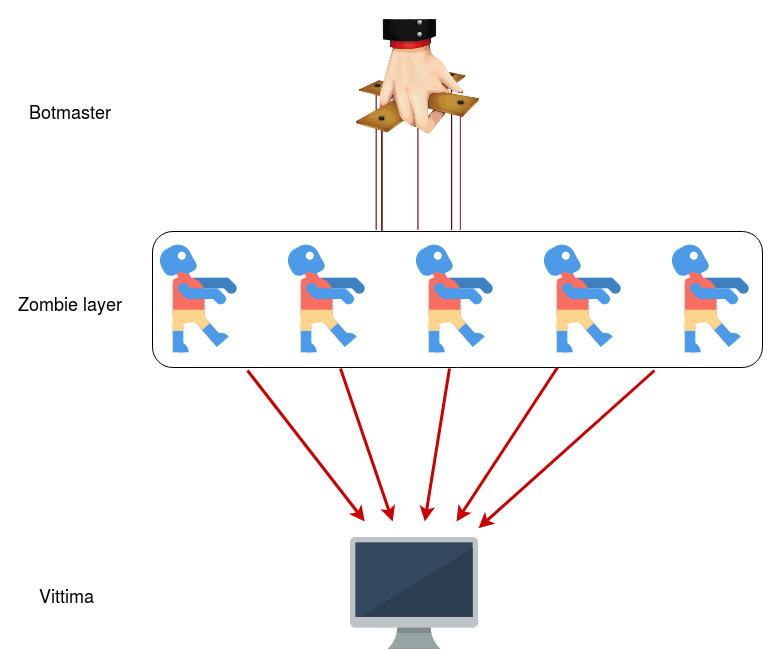
\includegraphics[scale=0.5]{zombielayer.png}
				\caption{Zombie layer}
\end{figure}

\section{Intrusion Detection and Prevention System}
Un'intrusione si verifica quando un aggressore tenta di entrare o interrompere le normali operazioni di un sistema informativo, quasi sempre con l'intento di fare del male \cite{idsbook}.
In questa sezione verranno presentati dei dispositivi utilizzati per identificare accessi non autorizzati ai computer o alle reti locali. Questi dispositivi possono essere utili per il rilevamento di botnet \cite{botnetdetection}.


I sistemi di rilevamento delle intrusioni sono gli "allarmi antifurto" del campo della sicurezza informatica. L'obiettivo è difendere un sistema con un allarme che viene emesso ogni volta che la sicurezza del sito è stata compromessa \cite{IDS}. 

Un IDPS è un dispositivo software o hardware utilizzato per identificare intrusioni a computer o reti locali.
Ci sono varie classi di intrusione che vanno rilevate: si possono verificare situazioni in cui un utente ruba una password, utenti legittimi che abusano dei loro privilegi o hacker che usano script trovati in rete per attaccare il sistema. Le intrusioni sono varie e non è possibile elencarle tutte.

Un IDPS è composto da quattro componenti \cite{idsbook}:

\begin{itemize}
				\item \textbf{Sensori}, sono utilizzati per ricevere informazioni dalla rete o dai computer.

				\item \textbf{Console}, utilizzata per monitorare lo stato della rete e dei computer.

				\item \textbf{Motore}, analizza i dati prelevati dai sensori e provvede a individuare eventuali falle nella sicurezza.

				\item \textbf{Database}, memorizza le regole utilizzate per identificare violazioni di sicurezza.
\end{itemize}

Di seguito è presente un'immagine che descrive i componenti di un IDPS. I pacchetti in entrata e uscita dalla rete sono ricevuti da un sensore che raccoglie il traffico dati, successivamente il motore analizza i dati prelevati dai sensori con le regole presenti nel database.

\begin{figure}[H]
				\centering
				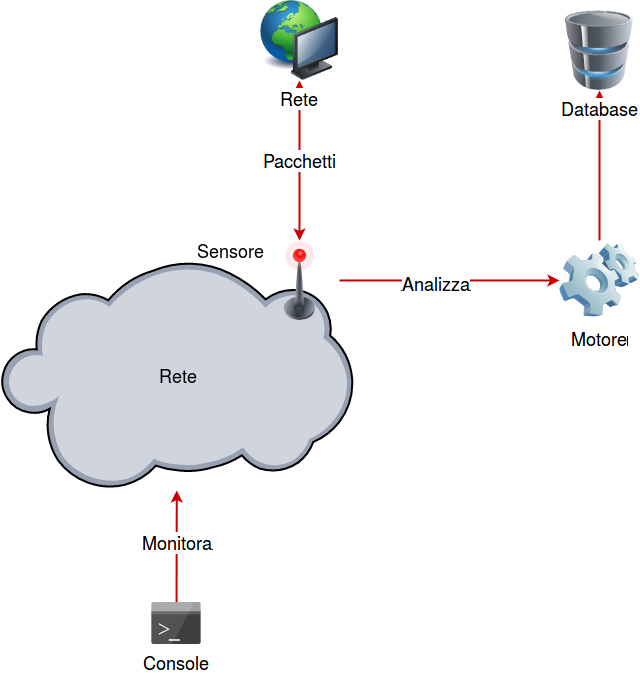
\includegraphics[scale=0.5]{IDS.png}
				\caption{Esempio di un IDS}
\end{figure}

Un'attuale estensione degli IDS sono i sistemi di prevenzione delle intrusioni detti IPS, che possono rilevare un'intrusione e impedire che l'intrusione attacchi con successo tramite una risposta attiva. Gli IPS usano diverse tecniche di risposte attive, che possono essere suddivise nei seguenti gruppi \cite{IPS}:

\begin{itemize}
				\item \textbf{terminare} la connessione internet o la sessione utente che sta eseguendo l'attacco
				\item \textbf{bloccare} l'accesso all'obiettivo e agli obiettivi simili all'utente o indirizzo IP che sta tentando un'intrusione
				\item \textbf{cambiare} l'ambiente di sicurezza modificando la configurazione di altri controlli di sicurezza per interrompere l'attacco, come la riconfigurazione delle regole di un firewall. Alcuni IPS possono anche applicare della patch di sicurezza a degli host se l'IPS rileva che l'host presenta delle vulnerabilità.
\end{itemize}

Poiché i due sistemi coesistono spesso, il termine combinato sistema di rilevamento e prevenzione delle intrusioni (IDPS) viene generalmente utilizzato per descrivere le attuali tecnologie anti-intrusione \cite{IPS}.


\subsection{Perchè usare IDPS}
Dispositivi di tipo IDPS sono utili per le difese di sistemi informatici per molteplici ragioni:
\begin{itemize}
				\item \textbf{defense in depth}, l'utilizzo di un dispositivo IDPS unito a firewall, controlli di accesso e autenticazione e antivirus permette la realizzazione di un meccanismo di protezione multi-livello
				\item \textbf{documentazione}, i dati acquisiti sono utili anche per il miglioramento continuo della qualità, gli IDPS raccolgono costantemente informazioni sugli attacchi che hanno compromesso con successo gli strati esterni dei controlli di sicurezza, per esempio di un firewall. Queste informazioni possono essere utilizzate per identificare e riparare le vulnerabilità esposte dagli attacchi, questo aiuta l'organizzazione ad accelerare il processo di risposta agli incidenti e ad apportare miglioramenti continui.
								Inoltre, nei casi in cui un IDPS non riesce a prevenire un'intrusione, può ancora assistere nella revisione fornendo informazioni su come si è verificato l'attacco, i dettagli su cosa ha fatto l'intruso e i metodi utilizzati. Gli IDPS possono anche fornire informazioni forensi che possono essere utili per motivi legali qualora l'attaccante venga catturato \cite{IPS}
				\item \textbf{insider threat}, gli attacchi non sempre arrivano dall'esterno, con questi dispositivi è possibile difendersi anche da intrusioni che avvengono all'interno della rete
\end{itemize}

Il miglior motivo per installare un IDPS è per la loro funzione di deterrente. Se gli utenti esterni e interni sanno che un'organizzazione ha un sistema di rilevamento e prevenzione delle intrusioni sono meno propensi a sondare o tentare di comprometterla \cite{IPS}.

\subsection{Tipi di IDPS}
Gli IDPS possono essere di due tipi in base al target su cui vengono applicati: possono essere basati su rete o su host. Un IDPS basato su rete è focalizzato sulla protezione delle risore di rete. Due sottotipi di IDPS basati su rete sono \cite{IPS}:

\begin{itemize}
				\item \textbf{wireless IDPS}, si concentra sulle reti wireless
				\item \textbf{network behavior analysis}, analizza i flow di traffico sulla rete nel tentativo di riconoscere dei modelli comportamentali anomali
\end{itemize}

Gli IDPS basati su host sono focalizzate sulla protezione dei server o dei singoli host.

\begin{verse}
				\textbf{Network-Based IDPS} Un IDPS basato sulla rete, detto NIDPS, è installato su un computer o dispositivo collegato ad un segmento della rete e ne monitora il traffico alla ricerca di indicazioni di attacchi. Un IDPS basato su rete può rilevare molti più attacchi rispetto ad un IDPS basato su host, ma richiede una configurazione e manutenzione più complessa. 
\end{verse}

\begin{verse}
				\textbf{Host-Based IDPS} Un IDPS basato su host, detto HIDPS, risiede su un particolare computer o server e monitora l'attività solo su quel sistema.
\end{verse}

\subsection{Metodi di rilevamento}

Gli IDPS utilizzano vari metodi di rilevamento per monitorare e valutare il traffico di rete. I metodi principali sono \cite{IDS}:

\begin{verse}
				\textbf{Signature detection} Questo metodo di rilevamento delle intrusioni esamina il traffico di rete alla ricerca di modelli che corrispondono a firme note, ovvero modelli di attacco preconfigurati e predeterminati. Questo metodo si basa sul presupposto che in qualsiasi caso riusciamo a definire un comportamento legale o illegale e a confrontarlo di conseguenza il comportamento osservato.
				Un vantaggio di questo approccio è che, avendo un modello con cui confrontare il comportamento che si sta osservando, non esistono falsi positivi. È inoltre veloce e semplice in quanto deve soltanto effettuare confronti con modelli illegali già noti.
				Uno svantaggio di questo approccio è che si possono verificare molti falsi negativi, cioè i comportamenti dannosi che non vengono segnalati. Questo si verifica perchè questi sistemi sfruttano regole per rilevare le intrusioni salvate su di un database, è quindi estremamente importante tenere aggiornato il database con tutti i possibili comportamenti dannosi.
\end{verse}

\begin{verse}
				\textbf{Anomaly detection} In questo tipo di rilevamento si parte con il presupposto che qualcosa di anormale sia molto probabilmente sospetto, si cercano quindi anomalie nel traffico. È quindi necessario uno studio anticipato della rete per capire cosa sia normale per il soggetto osservato. Si decide poi quanto è possibile discostarsi dal tipo di attività normale. Questo tipo di rilevamento guarda comportamenti che sono improbabili che si verifichino dallo studio effettuato sul traffico normale.  
				Il vantaggio di questo metodo è che indipendente dal tipo di intrusione ed è possibile utilizzare algoritmi di \textit{machine learning} che apprendono da soli cosa è normale osservando il traffico per un lungo periodo di tempo.
				Gli svantaggi sono la difficoltà di creare modelli e l'imprecisione che hanno questi modelli che danno vita a molti falsi positivi e falsi negativi.
\end{verse}

\section{Machine learning}
Il machine learning è un campo dell'intelligenza artificiale che si occupa di costruire programmi che migliorano con l'esperienza nell'eseguire un certo compito \cite{mldef}.

Questi tipi di algoritmi possono imparare e prendere decisioni in moto autonomo costruendo dei modelli dai dati passati in input.


Algoritmi di machine learning sono impiegati per compiti in cui la progettazione e la programmazione di algoritmi classici con buone prestazioni risultino difficili o addirittura impossibili. Per problemi come il riconoscimento vocale gli algoritmi basati sul machine learning superano tutti gli approcci che sono stati tentati fino ad oggi \cite{mldef}.
Applicazioni di esempio in cui è utilizzato il machine learning sono il filtro di mail considerate spam o il rilevamento di intrusi di rete.




I tipi di apprendimento automatico vengono classificati a seconda del segnale utilizzato per l'apprendimento o del feedback disponibile al sistema di apprendimento \cite{ai}.

\begin{verse}
				\textbf{Apprendimento supervisionato} Al computer vengono forniti degli esempi nella forma di possibili input e un valore di output, si vuole trovare quella funzione che dato un input non conosciuto calcola l'output. L'obiettivo è quello di fare una previsione basata su proprietà conosciute apprese dai dati in input.
\end{verse}

\begin{verse}
				\textbf{Apprendimento non supervisionato} Vengono forniti esempi con relative feature in input, ma non viene fornito alcun valore di output. L'obiettivo è scoprire nuove proprietà nei dati forniti in input.
\end{verse}

\begin{verse}
				\textbf{Apprendimento per rinforzo} Il computer impara interagendo con un ambiente dinamico nel quale cerca di raggiungere un obiettivo. L'insegnante gli dice solamente se ha raggiunto l'obiettivo. 
\end{verse}

\subsection{Apprendimento supervisionato}
In questa categoria di apprendimento vengono forniti esempi con relative feature in input e un valore di output. In base al valore di output si distinguono due diversi problemi:

\begin{itemize}
				\item \textbf{Classificazione} Se il valore di output è discreto, ad esempio l'appartenenza o la non appartenenza ad una determinata classe.
				\item \textbf{Regressione} Se il valore dell'output è un valore reale continuo in un determinato range.
\end{itemize}

In entrambi i problemi si vuole trovare una funzione \textit{h}, che dato un input non conosciuto stima il valore dell'output. L'obiettivo dei problemi di apprendimento supervisionato è quello di fare una predizione basata su proprietà conosciute apprese dai dai in input.
I dati in input vengono chiamati \textit{training set} e sono composti da un numero \textit{n} di esempi. Il valore di output è chiamato \textit{target value}.

La figura seguente descrive un problema di apprendimento supervisionato, dove l'algoritmo di apprendimento automatico prende in input un insieme di esempi da cui impara una funzione che gli permette di fare previsioni.

\begin{figure}[H]
				\centering
				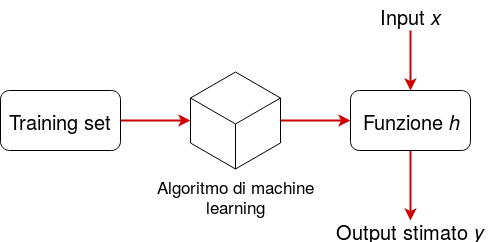
\includegraphics[scale=0.5]{apprendimentosupervisionato.png}
				\caption{Apprendimento supervisionato}
\end{figure}

\subsection{Apprendimento non supervisionato}
In questa categoria vengono forniti esempi con relative feature in input, ma non viene fornito alcun valore di output, quindi si hanno a disposizione dati non etichettati. L'obiettivo di questi algoritmi è quello di trovare delle strutture all'interno di questi dati non etichettati. Se si vogliono identificare dei raggruppamenti di elementi simili, è un problema di Clustering.

\begin{verse}
				\textbf{Clustering} È un tipico esempio di apprendimento non supervisionato in cui, dato un insieme di dati non etichettati, l'obiettivo è quello di individuare dei raggruppamenti, detti cluster, quanto più possibile coerenti.
\end{verse}	

\subsubsection{K-Means}
L'algoritmo K-Means è l'algoritmo di clustering più conosciuto e più utilizzato. Permette di suddividere un insieme di oggetti in $K$ gruppi sulla base dei loro attributi.

Si assume che gli attributi degli oggetti possano essere rappresentati come vettori, e che quindi formino uno spazio vettoriale. Dal \textit{dataset} fornito vengono inizializzati $n$ punti detti centroidi per ogni cluster che è necessario identificare.

Nell'esempio in figura vengono inizializzati due centroidi con una croce rossa e blu.

\begin{figure}[H]
				\centering
				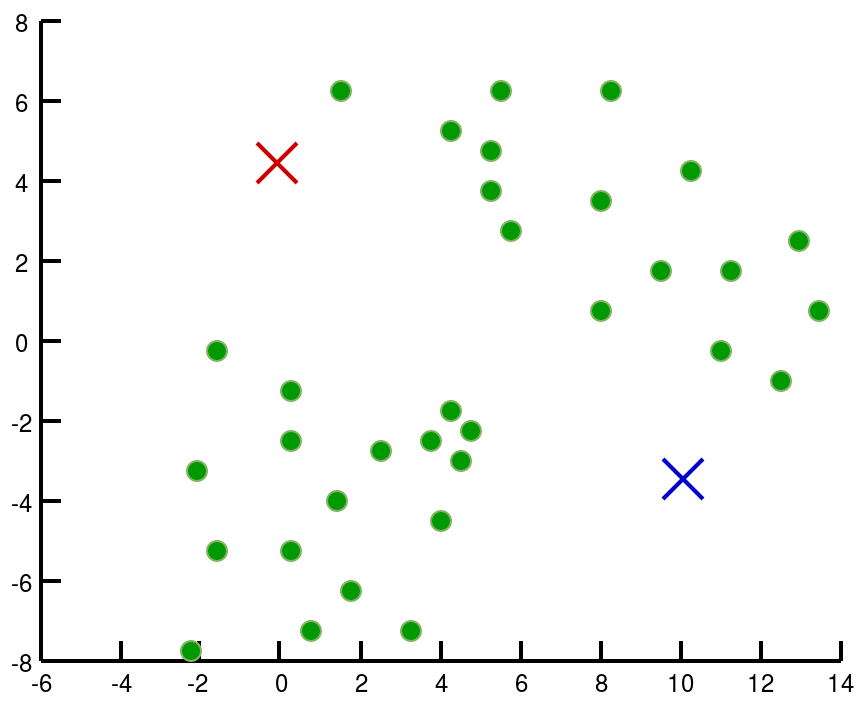
\includegraphics[scale=0.3]{k-means1.png}
				\caption{Algoritmo k-means - Inizializzazione}
\end{figure}

L'algoritmo segue una procedura iterativa che ripete due passi, il primo è il passo di assegnazione ai cluster, mentre il secondo è il passo di spostamento dei centroidi.
Il primo passo di assegnazione ai cluster controlla la distanza di ogni punto del dataset dai centroidi e assegna ciascun punto al centroide che gli è più vicino. 
L'esempio in figura rappresenta questo primo passo: i punti più vicini al centroide rosso sono stati colorati di rosso, mentre quelli più vicini al centroide blu sono stati colorati di blu.

\begin{figure}[H]
				\centering
				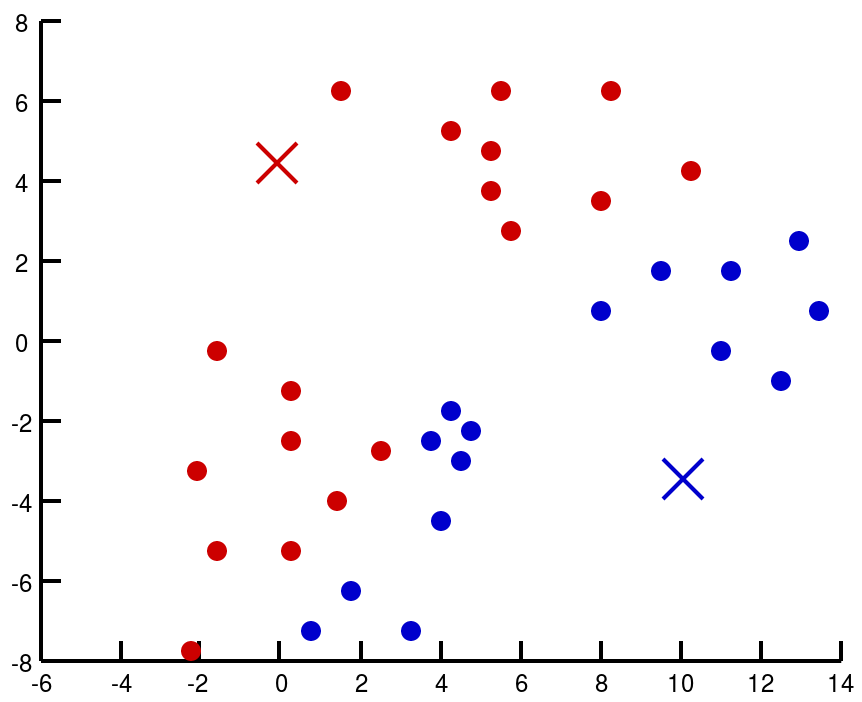
\includegraphics[scale=0.3]{k-means2.png}
				\caption{Algoritmo k-means - Passo 1}
\end{figure}

Il secondo passo consiste nel calcolare la media di tutti i punti nel dataset che appartendono ad un cluster e muovere in quella posizione il centroide del cluster.

\begin{figure}[H]
				\centering
				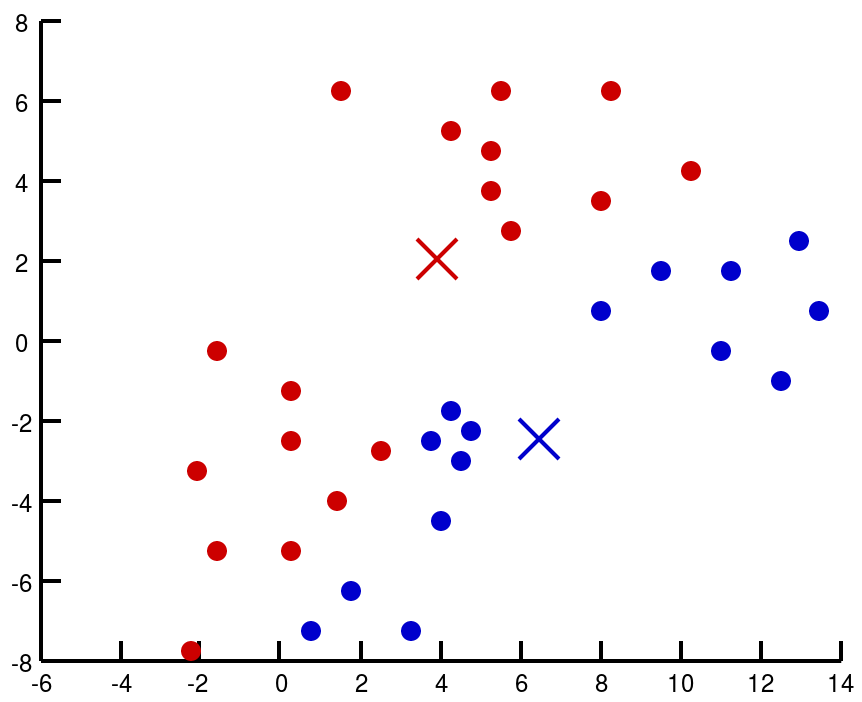
\includegraphics[scale=0.3]{k-means3.png}
				\caption{Algoritmo k-means - Passo 2}
\end{figure}

L'algoritmo continua a ripetere questi due passi fino a quando i centroidi non si spostano più, il che significa che l'algoritmo ha raggiunto la convergenza e i due cluster sono stati individuati.

\begin{figure}[H]
				\centering
				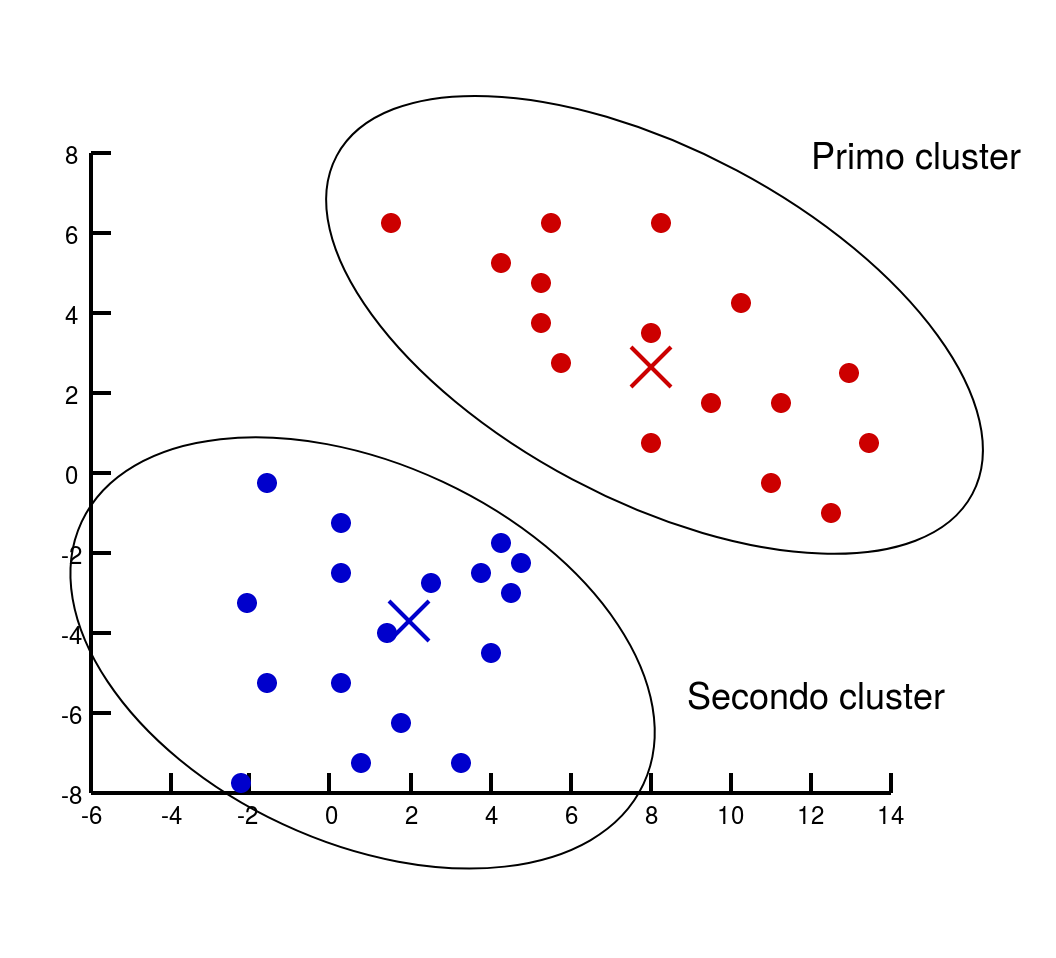
\includegraphics[scale=0.3]{k-means4.png}
				\caption{Algoritmo k-means - Convergenza}
\end{figure}






\end{document}
